\documentclass[pdf,notes]{beamer}
\mode<presentation>{\usetheme[secheader]{Boadilla}}

\usepackage{mystyle}
\includecomment{versiona}
\usepackage{xeCJK}
\usepackage{lpic}
\usefonttheme{professionalfonts}
\usepackage{etoolbox}

\newcommand{\red}[1]{{\color[rgb]{0.6,0,0}#1}}
\setbeamertemplate{theorems}[numbered] 

\usepackage{tikz}
\usetikzlibrary{shapes,arrows}
\newcommand{\Sol}{\mathcal{S}\mbox{ol}}
\newcommand{\Ind}{\mbox{\normalfont Ind}}
\newcommand{\Hom}{\mbox{\normalfont Hom}}
\newcommand{\D}{\mathcal{D}}
\newcommand{\A}{\mathcal{A}}
\newcommand{\Co}{\mathbb{C}}
\newcommand{\X}{\mathbb{X}}
\renewcommand{\setminus}{\backslash}
\newcommand{\nin}{\not\in}
\newcommand{\tmop}[1]{\ensuremath{\operatorname{#1}}}
\newcommand{\tmtextbf}[1]{{\bfseries{#1}}}
\newcommand{\tmtextit}[1]{{\itshape{#1}}}
\newcommand{\mss}{//}
\newcommand{\mbb}{\backslash\backslash}
\newcommand{\mmm}{\mid\mid}
\catcode`\<=\active \def<{
\fontencoding{T1}\selectfont\symbol{60}\fontencoding{\encodingdefault}}
\catcode`\>=\active \def>{
\fontencoding{T1}\selectfont\symbol{62}\fontencoding{\encodingdefault}}
\newcommand{\assign}{:=}
\newcommand{\comma}{{,}}
\newcommand{\um}{-}
\newcommand{\sol}{\mathcal{S}ol(\R^{p,q};\lambda,\nu)}
\newcommand{\Op}{\mbox{\normalfont Op}}
\newcommand{\Res}{\operatorname{Res}\displaylimits}
\newcommand{\OpR}{\mbox{\it R}}

%%\makeatletter
%%\newenvironment<>{proofs}[1][\proofname]{\par\def\insertproofname{#1\@addpunct{.}}\usebeamertemplate{proof begin}#2}
%%{\usebeamertemplate{proof end}}
%%\makeatother

\newtheorem{prop}{命題}
\newtheorem{remark}{注}

\AtBeginEnvironment{remark}{%
	    \setbeamercolor{block title}{bg=orange,fg=white}
		\setbeamercolor{block body}{bg=orange!20,fg=black}
}

\setCJKmainfont[AutoFakeBold=true]{Hiragino Mincho Pro} %my Mac

\title{2つのゲーゲンバウアー多項式に関連する積分公式について\footnote{60 min talk}}

% A subtitle is optional and this may be deleted

\author[レオンチエフ・アレックス]{小林俊行\inst{1} \and \underline{レオンチエフ・アレックス}\inst{2}}

\institute[東大] % (optional, but mostly needed)
{
  \inst{1}%
  大学院数理科学研究科、カブリ数物連携宇宙研究機構\\
  東京大学
  \and
  \inst{2}%
  大学院数理科学研究科\\
  東京大学
  }

  \date[表現論とその周辺分野の広がり]{RIMS共同研究(公開型)\\「表現論とその周辺分野の広がり」\\京都大学数理解析研究所}
% - Either use conference name or its abbreviation.
% - Not really informative to the audience, more for people (including
%   yourself) who are reading the slides online

\subject{表現論}

\begin{document}
\begin{frame}\titlepage\end{frame}

\begin{frame}{Outline}
	\tableofcontents
\end{frame}
\section{The integral formula related to two Gegenbauer polynomials}
\begin{frame}
	\begin{figure}[h]
		\centering
\begin{lpic}[]{wanted(0.75)}
	\lbl[bl]{3,15; \large$\begin{array}[]{c}
		\mbox{\it Expansion of $| s + t |^{2 \nu}$}\\\\\mbox{ in the form} \\\\
	| s + t |^{2 \nu} =	\\\\
	\sum_{\mbox{\scriptsize $\begin{array}[]{c}
\ell, m = 0 \\	 l + m\in2\N
\end{array}$}}^{\infty}
		a_{\lambda, \mu, \nu}^{\ell, m} C_{\ell}^{\lambda} (s) C_m^{\mu} (t)
	\end{array}$} %dot 
		
	\end{lpic}
		\label{fig:wanted}
	\vspace{-0.5cm}
		\caption*{Can we find the \underline{closed expression} for $a_{\lambda,\mu,\nu}^{\ell,m}$???}
	\end{figure}
\end{frame}
\begin{frame}
	\begin{prop}
		\begin{equation}
			| s + t |^{2 \nu} = \sum_{\mbox{\scriptsize $\begin{array}[]{c}
			\ell, m = 0 \\ \ell + m : \tmop{even}
		\end{array}$}}^{\infty} a_{\lambda,\mu,\nu}^{\ell,m} C_\ell^{\lambda} (s) C_m^{\mu} (t),
			\label{eqn:exp-st-gg}
		\end{equation}
		{\scriptsize
		\begin{equation*}
	a_{\lambda,\mu,\nu}^{\ell,m}= \frac{ 2^{-2\nu}(\lambda + \ell) (\mu + m)  \Gamma (\lambda + \mu + 2 \nu + 1) \Gamma (\lambda)
  \Gamma (\mu)\Gamma \left( 2\nu +
1 \right)}{\Gamma \left( \lambda + \nu + \frac{\ell -
  m}{2} + 1 \right)  \Gamma \left( \mu + \nu -
  \frac{\ell - m}{2} + 1 \right) \Gamma \left( \lambda + \mu + \nu + \frac{\ell +
  m}{2} + 1 \right)\Gamma\left(  \nu+1-\frac{\ell+m}{2}\right)}
		\end{equation*}
	}
	\end{prop}
	Here, $C_{\ell}^\lambda(t)$ ($\lambda\in\mathbb{C},\ell\in\N$) is the Gegenbauer polynomial.
	\begin{remark}
		We could not find this formula in the literature.
	\end{remark}
\end{frame}
\begin{frame}
	In fact, we can do more:
	\begin{prop}
		  \label{thm:4}For $\tmop{Re} \lambda, \tmop{Re} \mu > - \frac{1}{2}$,
		    $\tmop{Re} (\nu) > 0$ and $0 \leqslant z \leqslant 1$ the following holds:
		      \begin{eqnarray}
			          & | s + t z |^{2 \nu} \tmop{sgn}^{\frac{1 \pm 1}{2}} (s + t z) = \sum_{l,
					      m = 0 \mid l + m \equiv \frac{1 \pm 1}{2} \tmop{mod} 2}^{\infty} a_{l, m}
					          (z) C_l^{\lambda} (s) C_m^{\mu} (t), &  \nonumber\\
						      & a_{l, m} (z) = \frac{\Gamma \left( \nu + \frac{1}{2} \right) \Gamma
						      (\lambda) \Gamma (\mu) (\lambda + l) z^m }{(1 + \nu)_{- \frac{l + m}{2}} \sqrt{\pi} \Gamma
										      (\mu + m) \Gamma \left( \lambda + \nu + \frac{l - m}{2} + 1 \right)}&\nonumber
										      \\&\times{}_2 F_1 \left( \begin{array}{c}
								        \frac{l + m}{2} - \nu, \frac{m - l}{2} - \nu - \lambda\\
									      \mu + m + 1
									          \end{array} ; z^2 \right). & 
										          \nonumber
											    \end{eqnarray}
										    \end{prop}
\end{frame}
\section{Original motivation}
\begin{frame}
	\begin{block}{Goal:}
		\setbeamercolor{block title}{bg=red!30,fg=black}
		tesi me
	\end{block}
	\begin{block}{test}
		
	\end{block}
\end{frame}
\begin{frame}{How this is related to integral computation}
	Critical step in proving of Theorems 4--7 was the explicit computation of ``eigenvalues'' $C_{a',a,b}^{p,q}(\lambda,\nu)$.\footnote[frame]{I remember, You said the diagram is 
	too technical and better to be removed. I will do so in a subsequent versions, once I get it done. Nevertheless, I feel that it might be reused, so I'll type it in Tikz just in case. Any comments would be
appreciated.}\\
\begin{center}
	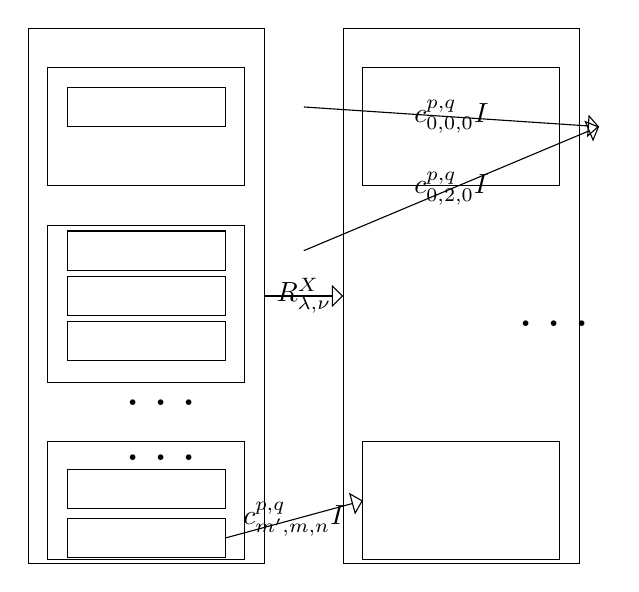
\begin{tikzpicture}
	\draw[color=black] (-9.0,0.75) rectangle (-6.0,-6.05);%upper
\draw[color=black] (-8.75,0.25) rectangle (-6.25,-1.25);%right in upper
\draw[color=black] (-8.5,0.0) rectangle (-6.5,-0.5);%in ``right in upper''
\draw[color=black] (-8.75,-1.75) rectangle (-6.25,-3.75);%middle in upper
\draw[color=black] (-8.5,-1.825) rectangle (-6.5,-2.325);%right in ``middle in upper''
\draw[color=black] (-8.5,-2.4) rectangle (-6.5,-2.9);%middle in ``middle in upper''
\draw[color=black] (-8.5,-2.975) rectangle (-6.5,-3.475);%left in ``middle in upper''
\draw[color=black] (-8.75,-4.5) rectangle (-6.25,-6.0);%left in upper
\draw[color=black] (-8.5,-4.85) rectangle (-6.5,-5.35);%right in ``left in upper''
\draw[color=black] (-8.5,-5.475) rectangle (-6.5,-5.975); %left in ``left in upper''

\draw[color=black] (-5.0,0.75) rectangle (-2.0,-6.05);%lower
\draw[color=black] (-4.75,0.25) rectangle (-2.25,-1.25);%right in lower
\draw[color=black] (-4.75,-4.5) rectangle (-2.25,-6.0);%left in lower

\node at (-7.25,-4.0) {\color{black}{\Huge \dots}};
\node at (-7.25,-4.7) {\color{black}{\Huge \dots}};
\node at (-2.25,-3.0) {\color{black}{\Huge \dots}};

%%\node at (-7.0,1.0) {\color{black}{$I(\lambda)$}};
%%\node at (-2.0,1.0) {\color{black}{$J(\nu)$}};

\draw[-open triangle 90] (-6.0,-2.65) to node {$R_{\lambda,\nu}^X$} (-5.0,-2.65);
\draw[-open triangle 90] (-5.5,-0.25) to node {$c^{p,q}_{0,0,0}I$} (-1.75,-0.5);
\draw[-open triangle 90] (-5.5,-2.075) to node {$c^{p,q}_{0,2,0}I$} (-1.75,-0.5);
\draw[-open triangle 90] (-6.5,-5.725) to node {$c^{p,q}_{m',m,n}I$} (-4.75,-5.25);

	\end{tikzpicture}
\end{center}
\end{frame}
\section{What does it have to do with?}
\end{document}


